\chapter{Theoretical Background}

\section{Feature Engineering}

Data mining is a machine learning tool that uses statistical methods to discover patterns in large datasets. Data mining has various stages to process knowledge and all of the stages run different methods to collect the appropriate data.

\begin{figure}[h]
	\centering
	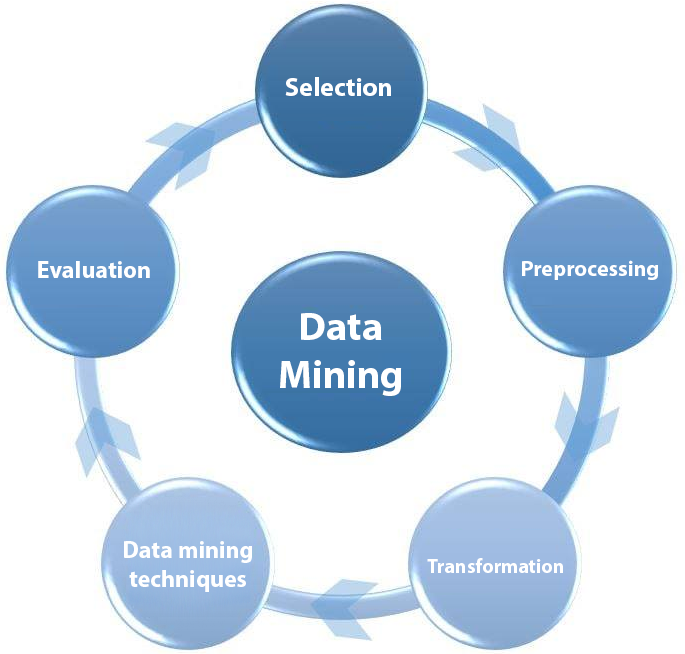
\includegraphics[height=0.55\linewidth]{./figures/data_mining_stages}
	\caption{Stages of data mining}
	\label{fig:stages}
\end{figure}

The first and most important part is to select the dataset which will be processed. \\
This means, that firstly the goal needs to be cleared up and then, depending on the problem, the information that seems to be useful for accomplishing the goal needs to be selected. In a dataset that processes real-world data, the selected features are always noisy and often contain faulty and inconsistent values. Hence data selection is a key factor to reach the most appropriate performance of the neural networks. 

\newpage
\noindent To decide the usefulness of a feature, the following quality requirements are assured: 
\begin{verse}
	$\bullet$ Validity: the degree to which the measures conform to defined business rules or constraints\\
	$\bullet$ Accuracy: the degree of conformity of a measure to a standard or a true value\\
	$\bullet$ Completeness: the degree to which all required measures are known\\
	$\bullet$ Consistency: the degree to which a set of measures are equivalent in across systems\\
	$\bullet$ Uniformity: the degree to which a set data measures are specified using the same units of measure in all systems
\end{verse}

There are some other criteria for the qualities of good features. A useful feature vector value appears more than one times in a dataset, which enables the model to learn the relationships between the feature vector values and the associated labels. This means having many examples with the same value helps the model to see the feature in different settings to determine when it is a good predictor. Also, each feature should have a clear and obvious meaning.


\subsection{Data Mining}

\textbf{Data preprocessing} \cite{pyle1999data} is a data mining technique that involves transforming raw data into an understandable format for computers. The selected dataset often includes errors, missing values or noisy, inconsistent data which have to be filtered during the preprocessing stage. \medskip

Data preparation and filtering steps can be time consuming. Data preprocessing includes cleaning, integration and reduction. Sometimes data transformation takes place in the preprocessing too. The product of data preprocessing is the final training set.\medskip

The given data in large datasets often contains information that is not clear enough. There are several techniques for repairing these uncertain data. \bigskip

\noindent For resolving missing values, the following steps can be taken:
\begin{verse}
	$\bullet$ Simply remove the feature vector, which is only effective if the vector contains several missing attributes.\\
	$\bullet$ Fill the missing values manually, which can be done with the mean value.
\end{verse}

Both techniques can create inaccuracies, but it is important to deal the appropriate technique, because the incorrect feature vector may contain necessary information too. \bigskip

Noise is a random error or variance in a measured variable. Noisy data needs to be smoothed to get the accurate prediction. Binning methods are local smoothing techniques, because they smooth the value with its neighbour's. Clustering can be used to detect outlier values by organizing them into similar groups. Data can be smoothed by fitting a function like regression to the data.\medskip

Data inconsistencies can be solved manually by external references, or with the use of knowledge engineering. Since the meaning of the features are given, it can be obvious to recognize an inconsistent value manually. Knowledge engineering uses technical, scientific and social aspects to deal with a feature value's inconsistency.\medskip

Data integration and reduction aims on the same goal to make the dataset clearer. During integration, an algorithm is looking through the dataset and looking for redundancies. \medskip

Data reduction is reducing the volume or the dimension of the dataset, without compromising the integrity of the original dataset. As the analysing can be time consuming, these data reduction techniques are really helpful in large datasets:\\
1. Dimension reduction: drop the irrelevant or weakly relevant values from the dataset\\
2. Data compression: use various encoding techniques to reduce the size of the dataset


\subsubsection{Transformation and Feature Scaling}

Some features of the dataset need to be transformed to get an appropriate form for data mining. Data transformation has a strong connection with \textbf{feature scaling} \cite{zheng2018feature, dong2018feature}, which is a statistical method used to standardize the range of the data. Feature scaling uses mathematical procedures to scale the range. 

\begin{figure}[h]
	\centering
	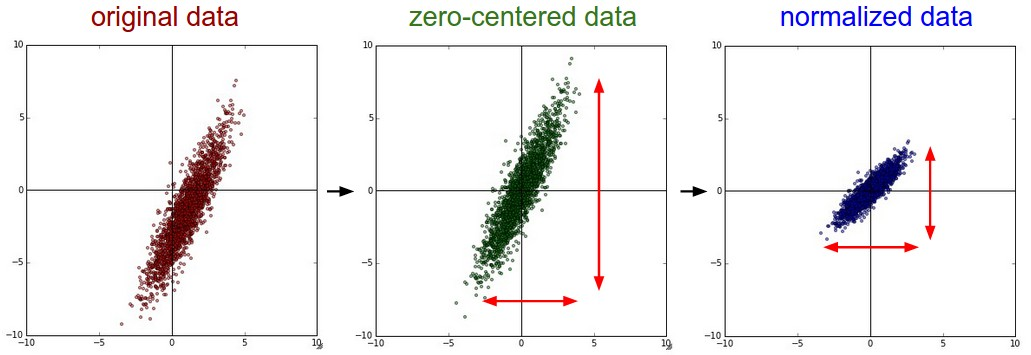
\includegraphics[height=0.35\linewidth]{./figures/data_mining}
	\caption{Data mining techniques can be used to convert data into understandable form.}
	\label{fig:data_mining}
\end{figure}

\textbf{Normalization} is the process of scaling individual samples to have a unit normal. Min-max scaling is the simplest normalization method that rescales the features to a range of $[0, 1]$ or $[-1, 1]$. The selected range depends on the data. It can be written as the following \autoref{eq:min-max}, where $x$ is the original, and $x'$ is the normalized value:
\begin{equation} x' = \frac{x-min(x)}{max(x)-min(x)} \label{eq:min-max} \end{equation} 

\smallskip \noindent Mean normalization in \autoref{eq:mean} is similar to min-max scaling, where $\bar x$ is the mean of $x$:
\begin{equation} x' = \frac{x-\bar x}{max(x)-min(x)} \label{eq:mean} \end{equation} \medskip

\textbf{Standardization} is the process of transforming the values of the given dataset into standard normality. Feature standardization in \autoref{eq:standard} gets the values of each feature to have zero-mean and unit-variance. 
\begin{equation}  x'= \frac{x-\bar x}{\sigma} \label{eq:standard} \end{equation}
where $x$ is the original feature vector, $\bar x$ is the mean of that feature vector and $\sigma$ is its standard deviation.\bigskip

\textbf{Encoding} is the process of converting data into an acceptable form for information processing. It can be used effectively on categorical features, because they use a set of values. \smallskip

Integer encoding converts the nominal values to numeric values. These numeric values are generally integers in increasing order, and they can cause inconsistencies with the given weights.\smallskip

One-hot encoding offers a solution for the inconsistency problem. It creates a binary vector for each categorical feature in the dataset where the values appears as follows:\\
$\bullet$ For those values which apply to the example, set the vector values to 1.\\
$\bullet$ Set other values to 0.\\
The length of the binary vector is equal to the number values in the current feature.


\subsubsection{Algorithms of Data Mining}

The algorithms of data mining originates from a wider field called \textbf{data analytics}. Data analytics is the process of examining datasets in order to draw conclusions about the information they contain. It focuses on processing and performing statistical analysis on existing datasets. The dataset is processed by data mining techniques that machine learning models can use. \medskip

The product of data mining is the training set. To apply data mining algorithms, the original dataset has to be split into multiple sets. The first one is called \textbf{training set}, which is used by the machine learning algorithm to gather knowledge and increase accuracy. The other one is the \textbf{testing set}, which is used to provide a dataset to test function estimation accuracy of the learning algorithm on the training dataset.\medskip

After the split, the following data mining techniques \cite{pujari2001data} can be used on the training set to discover patterns:\\
1. Classification: This method helps to retrieve information by classifying data into different classes. It can be used to draw further conclusions.\\
2. Clustering: It can be used to identify data which are similar to each other. It is an effective way to understand the similarities and differences between values.\\
3. Regression:  This method analyses the relationship between variables, to determine desired unknown values.\\
4. Association: It can discover hidden patterns in the dataset by identifying special events, for example high correlations between values.\\
5. Outlier detection: It collects outlier values which do not match an expected pattern or expected behavior. \\
6. Sequential Patterns: This method helps to identify similar patterns for a certain period. \\
7. Prediction: This method can be used for predicting future values in a dataset with the known of the given data and past events.  



\section{Regression Analysis}

Machine learning algorithms are able to use statistical techniques to predict the output values of a given dataset. Regression \cite{graybill1994regression} is a statistical technique, that adapts a function to the dataset to predict the values of a desired target variable. 

\begin{figure}[h]
	\centering
	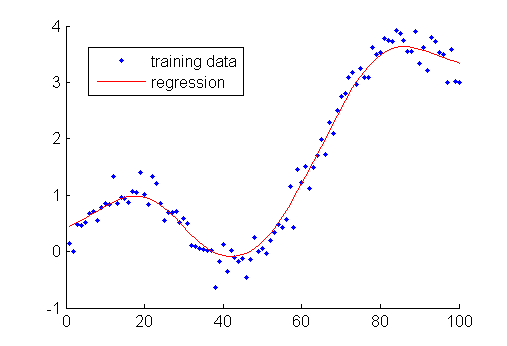
\includegraphics[height=0.42\linewidth]{./figures/regression}
	\caption{Regression is used to find the best fit of the training data by adapting a function to the dataset}
	\label{fig:regression}
\end{figure}

Regression analysis is a form of predictive modelling technique which investigates the relationship between one dependent variable, known as target, and a series of other independent variables, called predictors.  It also allows us to compare the effects of variables measured on different scales. \smallskip

\noindent Regression models involve the following parameters and variables:
\begin{verse}
	$\bullet$ The unknown parameters, denoted as $\beta\in\mathbb{R^\mathbb{N}}$, which may represent a scalar or a vector.\\
	$\bullet$ The independent variables: $X\in\mathbb{R}$.\\
	$\bullet$ The dependent variable: $y\in\mathbb{R}$.
\end{verse}

\noindent A regression model relates $Y$ to a function of $X$ and $\beta$ in \autoref{eq:regr}.
\begin{equation} y \approx f(X,\beta) \label{eq:regr} \end{equation}

Assume that the length of the vector of unknown parameters $\beta$ is $k\in \mathbb{Z}$. In order to perform a regression analysis, the information about the dependent variable $y$ must be provided:\smallskip

\noindent- If $N\in\mathbb{Z}$ data points of the form $(X,y)$ are observed, where $N<k$, most standard approaches of regression analysis cannot be performed as there are not enough data to recover $\beta$.\smallskip

\noindent- If exactly $N=k$ data points are observed, and the function $f$ is linear, the equations $y=f(X,\beta)$ can be solved. This reduces the problem to solving a set of $N$ equations with $N$ unknowns (the elements of $\beta$), which has a unique solution as long as the $X$ are linearly independent. If $f$ is non-linear, a solution may not exist, or many solutions may exist.\smallskip

\noindent- The most common situation is where $N>k$ data points are observed. In this case, there is enough information in the data to estimate a unique value for $\beta$ that best fits the data and the regression model when applied to the data can be viewed as an overdetermined system in $\beta$.\bigskip

Regression in connection with machine learning \cite{allen2007understanding} is a supervised learning task that can predict the output values of a desired target variable. In supervised learning tasks, the input and output values are both known and regression can be used when the data consist of continuous variables and real numbers.\smallskip

Since regression fits a function on a dataset, and the artificial neural networks can behave as a universal function approximator if there are infinite size of hidden layers available, neural networks can be used effectively to solve regression problems. Since there is no capacity for infinite number of neurons, the goal is to find that topology where the neural network is able to learn the regression function.


\subsection{Method of Least Squares}

In regression analysis, there is a standard approach called the method of least squares which approximates the solution of overdetermined systems and finds a solution for unknown parameters $\beta$.\medskip

The method of least squares or least squares fitting method \cite{wolberg2006data} is a mathematical procedure for finding the best-fitting curve to a given set of training data by minimizing the error. Error is the difference between the actual value of the dependent variable and the value predicted by the model. \medskip

Suppose that we have a series of $N\in\mathbb{Z}^+$ data points $(x_1, y_1), (x_2, y_2), \ldots, (x_N, y_N)$, where $x_i$ is an independent variable and $y_i$ is a dependent one. Also suppose that $x_1 < x_2 < \ldots < x_N$, i.e. the points are distinct and are in increasing order depending on $x$. The fit of a model to a data point is measured by the error $E_i$ in \autoref{eq:least1}:
\begin{equation} E_i=y_i-f(x_i,\beta) \label{eq:least1} \end{equation}
The method of least squares fitting aims to adjust the best-fitting values to the dataset. By performing least squares fitting algorithm, the required parameters $\alpha_1, \alpha_2, \ldots, \alpha_k$ of the function $f_{\alpha_1, \alpha_2, \ldots, \alpha_k} : [x_1, x_n] \rightarrow \mathbb{R}$ have been searched for, to minimize the sum $S$ of squared errors in \autoref{eq:least2}:
\begin{equation} S=\sum_{i = 1}^N ~ [f_{\alpha_1, \alpha_2, \ldots, \alpha_k}(x_i) - y_i]^2 \label{eq:least2} \end{equation}


\section{Perceptron}

A perceptron \cite{tho2010perceptron} is a single layer feedforward neural network, which has only one input and output layer. The perceptron's units are the artificial neurons, that are conventionally called nodes.\smallskip

In the input layer, each neuron has a weight connected to it, which represents the influence of that given neuron. The weights are used to decide the importance of the input values that are presented to the perceptron. Also the weights are used during the training of an artificial neural network as changing them in appropriate ways. If the predicted output is the same as the desired output, then the performance is considered satisfactory and no changes to the weights should be made. However, if the output does not match the desired output, then the weights need to be changed to reduce the error. \medskip

In order to avoid unnecessary iterations, it is important to adjust the weights in \autoref{eq:slp} properly.
\begin{equation} \Delta w = \eta * \hat{y} * x \label{eq:slp} \end{equation} 
where $\Delta w$ stands for the current weight, $\eta \leq 1$ is the learning rate which is the size of the required steps, $\hat{y}$ represents the desired output and $x$ is the input data. \medskip

To determine the value of a node, all the inputs would be multiplied by their respective weights, and then summed. This weighted sum stands for \textbf{dot product} in this context: $ z = w_1 x_1 + w_2 x_2 + \dots + w_m x_m = \sum_{j=1}^m w_j x_j $

\begin{figure}[h]
	\centering
	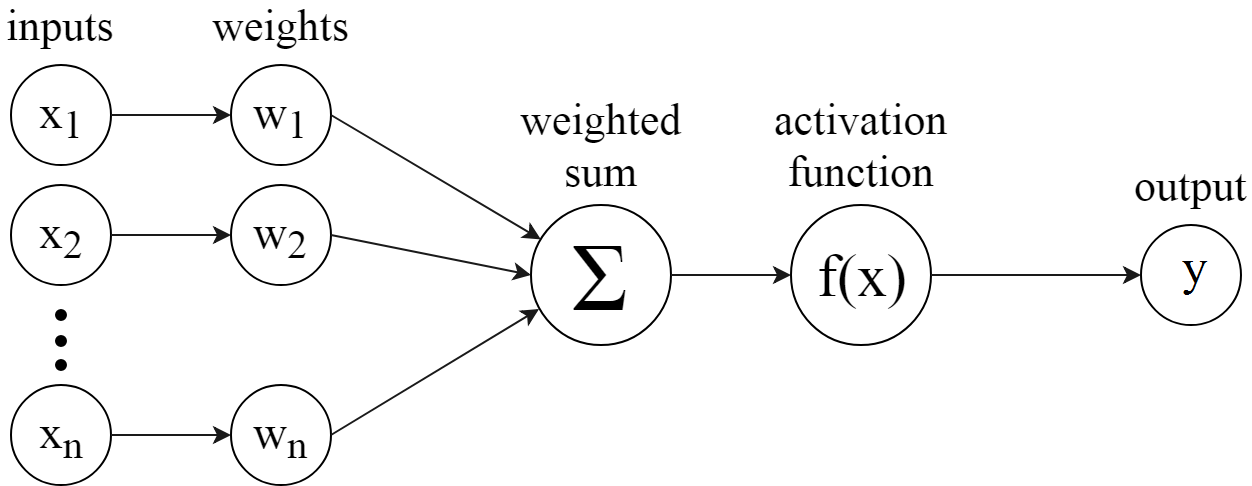
\includegraphics[height=0.28\linewidth]{./figures/perceptron}
	\caption{The appropriate weights are applied to the inputs and the resulting weighted sum passed to an activation function that produces the output.}
	\label{fig:perceptron}
\end{figure}

The output $y$ in \autoref{eq:slp-output} is determined by whether the weighted sum $\sum_j(w_j x_j)$ is less than or greater than some threshold value $\theta$, which is the parameter of the neuron. If that value is above a given threshold, it "fires", which means that the neuron gets an activated value. 
\begin{equation} y = \begin{cases} 0, & \hbox{for}~ \sum_j(w_j x_j) < \theta \\ 1, & \hbox{for}~ \sum_j(w_j x_j) \geq \theta \end{cases} \label{eq:slp-output} \end{equation} 

\newpage

\subsection{Feedforward Neural Networks}

The feedforward neural network \cite{fine2006feedforward} is a type of neural networks, which aims to create a mapping from a properly trained input dataset to an estimated output. This type of neural network is called feedforward as there are no feedback connections in which outputs of the neuron are connected to itself. A feedforward neural network is able to model complex non-linear functions. 

\begin{figure}[h]
	\centering
	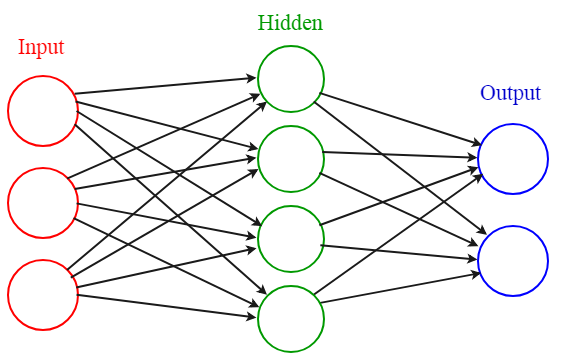
\includegraphics[height=0.35\linewidth]{./figures/feedforward}
	\caption{A feedforward neural network, that does not contain any feedback connections between the nodes.}
	\label{fig:feedforward}
\end{figure}

A typical feedforward neural network consists of input and output layers. There is an intermediate part between inputs and outputs, called hidden layers. The \textbf{input layer} is a set of input neurons, where each neuron represents a feature in our dataset. The \textbf{output} of any feedforward network is the sum of the inputs multiplied by the weights. The \textbf{hidden layer} contains units which can transform the inputs into a mapping that the output layer can utilize. The relationship between the input and hidden layer is determined by the weights of the network. \bigskip

\noindent The output of a trained feedforward neural network can be characterized by the \autoref{eq:feedforward}
\begin{equation} y_k = f_k(i,w) \label{eq:feedforward} \end{equation}
where $y_k$ means the $k$th neural network output, $(i,w)$ is a vector of the weights and $f_k(\cdot)$ describes the mapping from the input to the $k$th output, where $f_k(\cdot)$ also contains the structure of the feedforward perceptron. The neural network can be trained if the input and the output are fixed and the weights are adjusted. When a single scalar output can be found, $y_k$ can be replaced by $y$ and $f_k(\cdot)$ by $f(\cdot)$.



\subsection{Multi-Layer Perceptron}

The multi-layer perceptron is a multi-layered feedforward neural network algorithm that learns a function $f(\cdot) : \mathbb{R}^m \mapsto \mathbb{R}^n$ by training on a dataset, where $m$ is the number of dimensions for the input and $n$ is the number of dimensions for the output. Given a set of features $X = x_1, x_2, \dots, x_m$ and a target $y$, it can be a non-linear function approximator for either classification or regression. \medskip

The difference between single- and multi-layered neural networks is that the multi-layered perceptron has one or more hidden layers besides the input and output layer. Except for the input nodes, each node is a neuron that uses a linear or non-linear activation function. \medskip

The process of making a multi-layer neural network is simple with the use of the perceptrons.\\
1. Assume that there are $m\in\mathbb{Z}$ features in input $X$, so $m\in\mathbb{Z}$ weights are needed to perform a dot product.\\
2. With $n$ hidden neurons in the hidden layer, $n\in\mathbb{Z}~$ sets of weights $(w_1, w_2, \dots , w_n)$ are needed for performing dot products.\\
3. With one hidden layer, $n$ dot products can be performed to get the hidden output $h: (h_1, h_2, \dots , h_n).$\\
4. Then the hidden output that also has $n$ features can be used as input data to perform dot product with a set of $n$ weights and get the final output $y$. \bigskip

In a multi-layer perceptron, each neuron in one layer is connected with a weight to another neuron in the next layer. Each of these neurons stores a value, which is in general a sum of the weighted neurons which comes from previous layers. There is a special unit, called \textbf{bias}, that are not influenced by any values in the previous layer, so they do not have any incoming connections. However they have outgoing connections and they can contribute to the output of the artificial neural network. Bias units stores a constant value, which helps the model to fit the best for the given data. Hence the definition of dot product expands like the \autoref{eq:mlp}:
\begin{equation} z = \sum_{j=1}^m w_j x_j + bias \label{eq:mlp} \end{equation}

Neural networks are designed to learn from datasets by using iterative methods. Estimation value error is calculated from the desired and the predicted values to modify the weights of the connections between neurons. A multi-layer perceptron utilizes a supervised learning technique called \textbf{backpropagation} for training.


\subsubsection{Backpropagation}

The main goal of backpropagation \cite{chauvin2013backpropagation} is to update all of the weights in the neural network, in such way that the predicted output to be closer to the target output while minimizing the error of each output neuron and the network.

The algorithm consists of two phases: the forward phase where the activations are propagated from the input to the output layer, and the backward phase, where the error between the actual and the desired value in the output layer is propagated backwards to modify the weights values. \medskip

Assume that $N$ is a neural network with $e$ connections, $m$ inputs, and $n$ outputs, where $N,e,m,n\in\mathbb{Z}$. Below, $x_{1},x_{2},\dots$ will denote vectors in $\mathbb{R}^m$, $y_1,y_2,\dots$ vectors in $\mathbb{R}^n$, and $w_0,w_1,w_2,\dots$ vectors in $\mathbb{R}^e$. These are the inputs, outputs and weights, respectively. The neural network corresponds to a function $y=f_N(w,x)$, which gives a weight $w$ and maps an input $x$ to an output $y$. The optimization takes a sequence of training examples $(x_1,y_1),\dots ,(x_p,y_p)$ and produces a sequence of weights $w_0,w_1,\dots ,w_p$ starting from an initial weight $w_0$ that is usually chosen at random. Then first compute $w_i$ using only $(x_i,y_i,w_{i-1})$ for $i=1,\dots ,p$. The output of the algorithm is $w_p$, giving us a new function $x \mapsto f_N(w_p,x)$. The computation is the same in each step, so only the case $i=1$ is described. Calculating $w_1$ from $(x_1,y_1,w_0)$ is done by considering a variable weight $w$ and applying gradient descent to the function $w \mapsto E(f_N(w,x_1),y_1)$ to find a local minimum, starting at $w=w_0$, where $E$ is the error function. This makes $w_1$ the minimizing weight found by gradient descent.\medskip

The function that is used to compute this error is known as \textbf{loss function}. For backpropagation, the loss function calculates the difference between the network output and its expected output, after a training example has propagated through the network. \medskip

Different loss functions will give different errors for the same prediction, and thus have a considerable effect on the performance of the model. In the training of multi-layer perceptrons, L2 loss function $L$ has been used in \autoref{eq:backprop}, which is the square of the L2 norm of the difference between actual value $y$ and predicted value $\hat{y}$.
\begin{equation} L = \sum^n_{i=1}(y_i - \hat{y})^2 \label{eq:backprop} \end{equation}



\subsubsection{Gradient descent}

One generally used method used for backpropagation in the calculation of the weights is gradient descent \cite{anderson1995introduction}. It is an optimization method, which aims to minimize a given function to its local minimum by iteratively updating the weights of the model. The input is defined with an initial value and the algorithm calculates the gradient i.e. the partial derivative of the loss curve at this starting point. Gradient descent can be used to solve a system of linear and non-linear equations too, but only the linear one will be explicated in \autoref{eq:lin_grad}:
\begin{equation} \hat{y} = wx + b \label{eq:lin_grad} \end{equation}
where $x$ is the input, $\hat{y}$ is the predicted output, $w$ defines weights and $b$ stands for bias.\medskip

In the operation of gradient descent, cost function $f(w,b)$ in \autoref{eq:cost} utilizes the value of the loss function to define how to update our weights to make the model more accurate.
\begin{equation} f(w,b) ~~=~~ \frac{1}{n} \sum_{i=1}^n(y_i-\hat{y})^2 ~~=~~ \frac{1}{n} \sum_{i=1}^n(y_i-(wx_i+b))^2 \label{eq:cost} \end{equation}

From the cost function, the partial derivatives of the cost function are calculated with respect to each parameter and results are stored in a gradient in \autoref{eq:partial}.
\begin{equation} f'(w,b) = \bmatrix{ \aligned \frac{\partial f}{\partial w} \\
	\frac{\partial f}{\partial b} \endaligned }\endbmatrix
= \bmatrix{ \aligned \frac{1}{n} \sum - 2x_i(y_i-\hat{y}) \\
	\frac{1}{n} \sum - 2(y_i-\hat{y}) \endaligned }\endbmatrix \label{eq:partial} \end{equation}

\noindent Thus the process of the gradient descent algorithm is the following:\\
1. Initialize the weights with an initialize value and calculate the cost function.\\
2. Calculate the gradient, i.e. change the weights a bit from their original initialized value to the direction in which the cost function is minimized.\\
3. Adjust the weights with the gradients to reach the optimal values where $f(w,b)$ is minimized.\\
4. Use the new weights for prediction and to calculate the new cost function.\\
5. Repeat steps 2, 3 until the adjustments to weights does not significantly reduce $f(w,b)$.\bigskip

\noindent In \autoref{fig:gradient} the components of gradient descent are the following:
\begin{verse}
	$\bullet$ Learning rate: size of steps took in any direction\\
	$\bullet$ Gradients: the direction of the steps, i.e. the slope\\
	$\bullet$ Cost function: tells the current height, which is the sum of squared errors
\end{verse}

\begin{figure}[h]
	\centering
	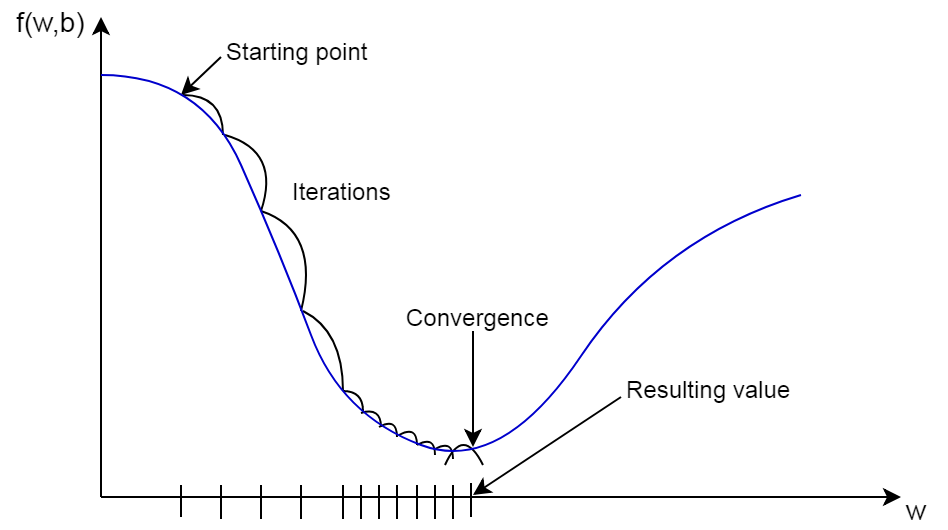
\includegraphics[height=0.4\linewidth]{./figures/gradient}
	\caption{The gradient descent is an optimization method used by backpropagation}
	\label{fig:gradient}
\end{figure}

In backpropagation, the calculation of the gradient passes the network backwards, so the values of the gradient from one layer are reused in the computation of the gradient for the previous layer. 




\section{Training a MLP Model}

The task that is being tackled in this thesis is to make the inversion of a single element feedforward neural network. To eventuate this successfully, the appropriate dataset is given and already preprocessed. Hence the main task is now to train a neural network to predict new outputs for the testing set and minimize the loss between the given and the desired outputs from the training set. The method is given by backpropagation, but there are a lot of components of the neural network model that plays a very important role in the effective training to produce accurate results. These components are the activation function, optimization algorithm, the appropriate topology i.e. the size of the layers, the learning rate, and so on. Different tasks require a different set of functions to give the most optimum results. The used methods and functions are described in the following subsections.


\subsection{Activation Functions}

In connection with artificial neural networks, the activation function is a transitional state of the neurons between other layers. It is a mapping of the previous layers and it maps the resulting value into the desired range, which is usually between -1 and 1. The output of the activation function is then used as input for the next layer, until a desired solution is found. There are several activation functions, and each of them utilizes different methods for mapping. \medskip

As the multi-layer perceptron approximates non-linear functions, it will be the most accurate by using non-linear activation functions as well \cite{pillo2013nonlinear}. These non-linear activation functions are known for having more than one degrees and have a curve in their graph. As non-linear functions can generate non-linear mappings from inputs to outputs, they can be applied on complex datasets. 

\begin{figure}[h]
	\centering
	\caption{The graphs of the most popular non-linear activation functions}
	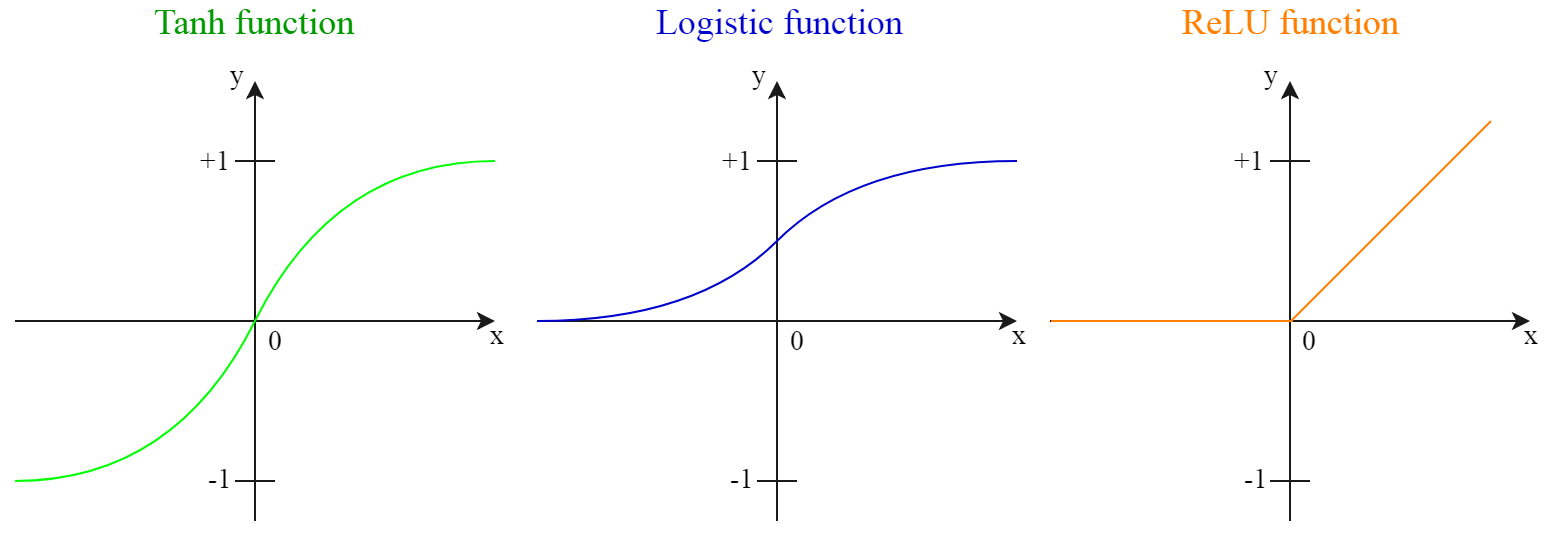
\includegraphics[height=0.35\linewidth]{./figures/functions}
	\label{fig:functions}
\end{figure}

\bigskip \noindent The two common non-linear activation functions are both sigmoids, as they approximate with a curve instead of a straight line. These are the \textbf{hyperbolic tangent} and the \textbf{logistic} functions, described by \autoref{eq:activation}
\begin{equation} f(x)=tanh(x) ~~~~~ \hbox{and} ~~~~~ f(x)=\frac{1}{1+e^{-x}} \label{eq:activation} \end{equation}
The hyperbolic tangent ranges from -1 to 1, while the logistic function is similar in shape but ranges from 0 to 1. \medskip

The \textbf{ReLU} function is another type of non-linear functions, which stands for rectified linear unit. It is called half-rectified, because no negative values are allowed. This operation affects the resulting graph (\autoref{fig:functions}), as the negative values are shown as zeros in \autoref{eq:activation2}.
\begin{equation} f(x) = max(0,X) \label{eq:activation2} \end{equation}



\subsection{Optimization Methods}

Artificial neural networks have different phases in the process of their operation. The learning process in a neural network uses different training methods with different characteristics and performance. These training methods use optimization algorithms to update weights and biases i.e. the internal parameters of a model to reduce the error. \cite{veerarajan2007numerical, sathasivam2003optimization}



\subsubsection{Stochastic Gradient Descent}

Stochastic gradient descent is a stochastic approximation of gradient descent optimization, used effectively in large-scaled datasets. In contrast to gradient descent, the stochastic method can approximate the true gradient of the cost function because it updates the parameters for each training example, one by one. \smallskip

To demonstrate assume that $\eta$ is the learning rate, $L$ stands for the loss function and $\nabla_w L = \frac{\partial L}{\partial w}$ is the gradient. Now the updating equation of the weights $w$ in each iteration is:
\begin{equation} w_{t+1} = w_t - \eta \nabla_w L \label{eq:sgd} \end{equation} 

\noindent The process of the stochastic gradient descent algorithm is the following:\\
1. Choose one sample from the dataset (this is what makes it stochastic gradient descent).\\
2. Calculate all the partial derivatives of loss with respect to weights or biases. \\
3. Use the update \autoref{eq:sgd} to update each weight and bias.\\
4. Go back to step 1.

\begin{figure}[h]
	\centering
	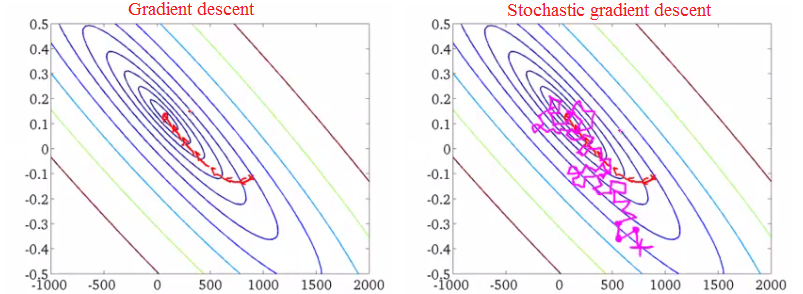
\includegraphics[height=0.28\linewidth]{./figures/stochastic}
	\caption{The difference between the process of GD and SGD methods}
	\label{fig:stochastic}
\end{figure}


\subsubsection{Adaptive Moment Estimation}

Another method is adaptive moment estimation, called Adam. This brand-new optimization method is designed to solve deep learning problems. Adam is a transition between adaptive methods and momentum-based methods. In the algorithm, running averages of both the gradients and the second moments of the gradients are used, which means Adam not only stores the exponentially decaying average of past squared gradients $v_t$, it also keeps the decaying average of past gradients $m_t$, similarly to momentum-based methods. The algorithm computes the decaying averages of past $m_t$ and past squared $v_t$ gradients respectively as follows in \autoref{eq:adam1}:
\begin{equation} m_t = \beta_1 m_{t-1} + (1-\beta_1)L_t ~~~~\hbox{and}~~~\ v_t = \beta_2 v_{t-1} + (1-\beta_2)L^2_t \label{eq:adam1} \end{equation}
where $m_t$ and $v_t$ are the estimates of the first and second moments, $\beta_1$ and $\beta_2$ are the decay for gradients and second moments of gradients, and $L_t$ is the loss function.\\
The first and second moment estimates are in \autoref{eq:adam2}:
\begin{equation} \hat{m_t} = \frac{m_t}{a-\beta^t_1} ~~~~\hbox{and}~~~ \hat{v_t} = \frac{v_t}{a-\beta^t_2} \label{eq:adam2} \end{equation}
Then these estimates are used to update the parameters $w$ with a simple scalar $\epsilon$ to prevent division by 0 in \autoref{eq:adam3}:
\begin{equation} w_{t+1} = w_t - \frac{\mu}{\sqrt{\hat{v_t}}+\epsilon}\hat{m_t} \label{eq:adam3} \end{equation}


\subsubsection{Limited-memory BFGS}

Limited-memory BFGS - against the previous ones - is a quasi-Newton method for weight optimization, that uses Hessian matrices to approximate. L-BFGS originates from the Broyden–Fletcher–Goldfarb–Shanno algorithm with limited amount of computer memory. L-BFGS aims on parameter estimation, and the target problem is to minimize $f(x)$ over unconstrained values of the real-vector $x$ where $f$ is a differentiable scalar function. In this method, the Hessian matrix of second derivatives is not computed, just approximated by using gradient evaluation updates. \medskip

\noindent From an initial guess $x_0$ and an approximate Hessian matrix $B_0$, the following steps are repeated as $x_k$ converges to the solution:\\
1. Obtain a direction $p_k$ by solving $B_k p_k = - \nabla f(x_k). $ \\
2. Perform a one-dimensional optimization to find an acceptable stepsize $\alpha_k$ in $p_k$. \\
3. Set $s_k = \alpha_k p_k$ and update $x_{k+1} = x_k + s_k.$ \\
4. Set $y_k = \nabla f(x_{k+1}) - \nabla f(x_k).$ \\ 
5. The solution is $B_{k+1} = B_k + \frac{y_k y^T_k}{y^T_k s_k} - \frac{B_k s_k s^T_k B_k}{s^T_k B_k s_k}.$

\begin{figure}[h]
	\centering
	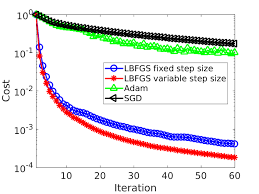
\includegraphics[height=0.36\linewidth]{./figures/optimization}
	\caption{The optimization of SGD, Adam and L-BFGS with respect of cost and iteration}
	\label{fig:optimization}
\end{figure}



\section{Inversion}

The inverse of a function means the reverse of another function in mathematics. For a given $f: X \mapsto Y$, the inverse function of $f$ is that $g: Y \mapsto X$, where $f(x) = y$ and $g(y) = x$. Thus $g = f^{-1}$. \medskip

Not all of the functions are invertible. The inverse of a function exists, if that function is \textbf{injective}, so there are another function with which they preserve distinctness. This means a one-to-one mapping. However injectivity only provides that every $x$ in $X$ maps to a $y$ in $Y$. But also it is not a criteria that all of the elements in $Y$ belongs to an $x$, so here some $y$ may exist which are not a mapping of any $x$.

\begin{figure}[h]
	\centering
	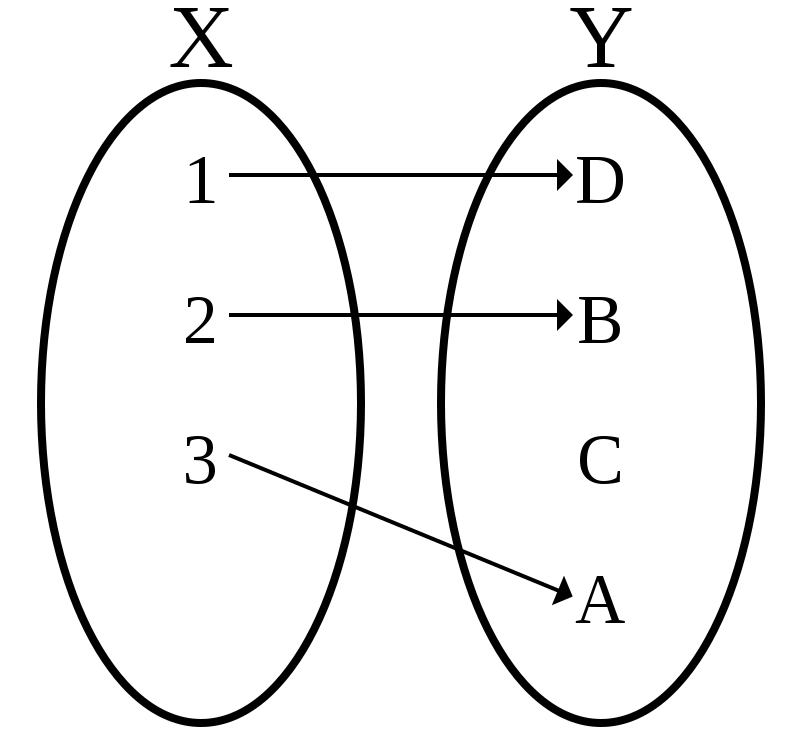
\includegraphics[height=0.23\linewidth]{./figures/injection}
	\caption{Injective function means a one-to-one mapping from $X$ to $Y$.}
	\label{fig:injective}
\end{figure}

\label{para:surj}In case of \textbf{surjection}, for every $y$ in $Y$ there is a mapping from an $x$ in $X$. Also, $x$ do not has to be unique, so more $x$ can map to the same $y$.

\begin{figure}[h]
	\centering
	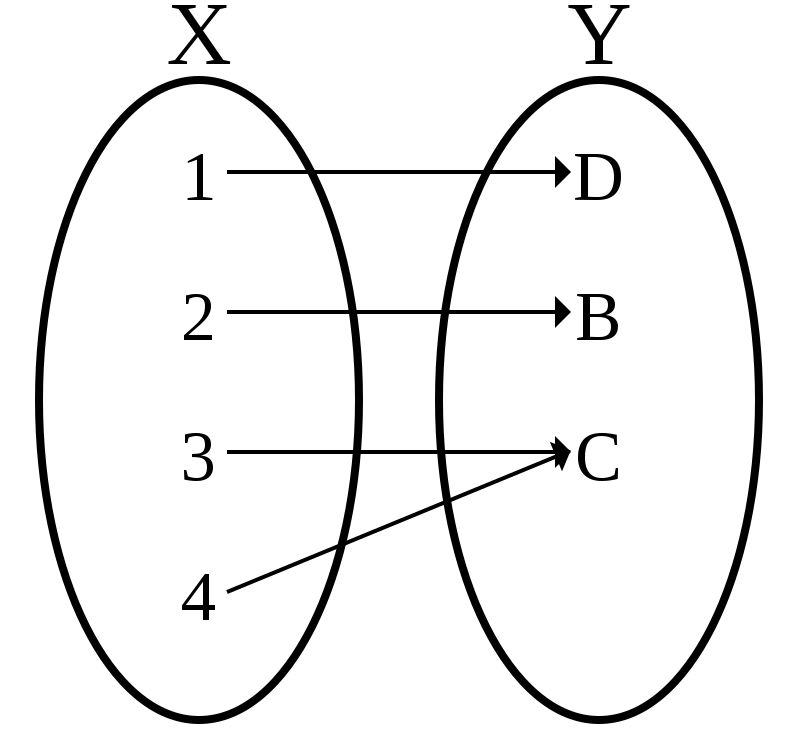
\includegraphics[height=0.23\linewidth]{./figures/surjection}
	\caption{In case of surjection, more $x$ can map to the same $y$.}
	\label{fig:surjective}
\end{figure}

If a function is \textbf{bijective}, it is injective and surjective at the same time, so every $x$ corresponds to one, and only one $y$, where $X, Y \in \mathbb{Z}^+$ and the number of elements are equal in $X$ and $Y$. 

\begin{figure}[h]
	\centering
	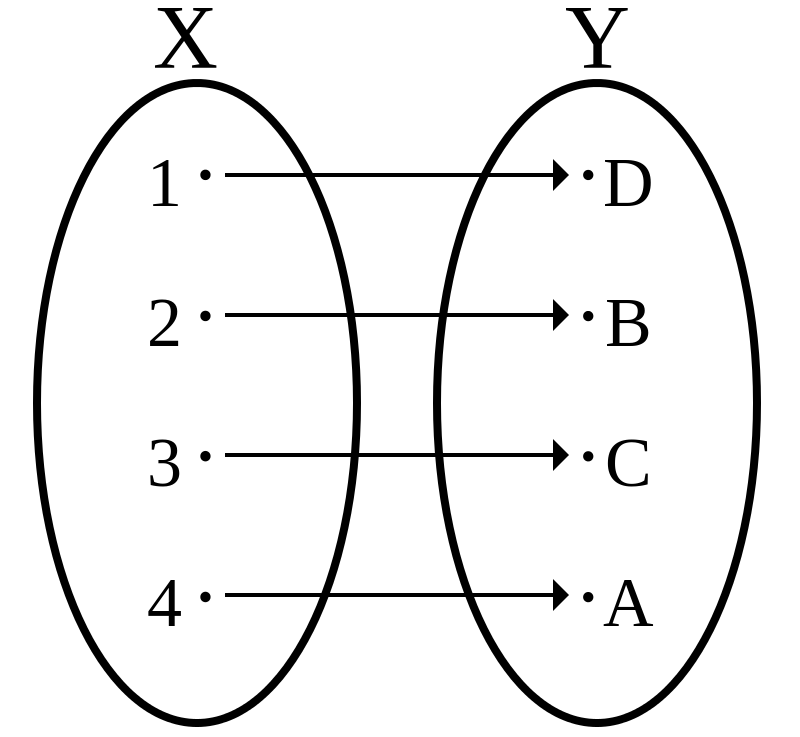
\includegraphics[height=0.23\linewidth]{./figures/bijection}
	\caption{If a function is bijective, every $x$ corresponds to one, and only one $y$.}
	\label{fig:bijective}
\end{figure}

Bijective functions are mutually unequivocal, so they can be mapped back and forth. When it is fulfilled, it can be said that the given $f(x) = y$ is mappable so that $g(y) = x$. Simply a function $f$ has an inverse function, if for every $y$ in $Y$ that there must be one, and only one $x$ in $X$ so that $f(x) = y$.\bigskip

Since artificial neural networks can behave as a universal function approximator, the inversion of a neural network is meant to be a process, which consists of clamping the weights and the neural network output while adjusting the input in the neural network until an equality or a best possible fit occurs for one or more values of the input. \medskip

Feedforward neural networks aim on to capture system mapping from the given training data. The goal is to find the input values that will result the desired output for the given weights. The problem is that in case of a dataset, bijection is not guaranteed, since the output values are just rarely unique. Generally it can be determined that numerous inputs can generate the same output (seen at surjection in \ref{para:surj}). So the neural networks are literally not invertible, but in case of a sufficient number of data with the assistance of a properly big topology, neural networks are able to estimate the inputs quite accurately for the examined output.

\bigskip \noindent The process of finding the inversion $f^{-1}(x)$ of a function $f(x)$ is the following:\\
1. Replace $f(x)$ with $y$.\\
2. Replace every $x$ with a $y$ and replace every $y$ with an $x$. \\
3. Solve the equation from step 2 for $y$. \\
4. Replace $y$ with $f^{-1}(x)$. 



\subsection{Single Element Inversion Methods}

In case of single element inversion, one single point can be estimated in every iteration from the input set in respect of the given output. It's accuracy is depending on the initialization and it will result a nearer outcome in further processes. However not the only important task is to find the best topology, but also to find a properly training algorithm, because it notes the previously founded points and reuses them. The process of finding the best estimator is time consuming. As the quantity of parameter combinations increases during the training phase, so does the time that the training takes. However, the number of parameter combinations also potentially increase the inversion accuracy.\bigskip

To solve the inversion of an unconstrained optimization problem, the inversion method needs to solve the optimization itself in its training phase. After the dataset is properly trained, the inversion problem is the following:\medskip

Given some neural network function $f : X \mapsto Y$, for some $y \in Y$, the appropriate $x \in X$ needs to be found, such that $f(x) = y$. Or more generally, if $L : Y \mapsto \mathbb{R}$ is the loss function defined over the network output, an input $x$ have to be found that minimizes $L(f(x))$. 


\subsection{Williams-Linder-Kindermann Inversion}

\label{para:wlk-inv}The WLK inversion was named after R. L. Williams, A. Linder and J. Kindermann \cite{KINDERMANN1990277}, who firstly introduced the single element search method for inversion of real valued neural network. In this algorithm, the inversion problem is set up as an unconstrained optimization problem and solved by gradient descent, similarly to backpropagation. \medskip

\noindent The method of WLK inversion involves two main steps: \\
1. computing the deltas for every value \\
2. updating the weights manually \bigskip

During the training, the neural network is trained to learn a mapping from input to output. The proper set can be find by minimizing the loss. Thus the neural network learns a functional relationship between the inputs and the outputs. Now all the weights are fixed. \medskip

Assume that the initial input vector $i_0$ is given. Now the recursive equation of the training phase is the following: 
\begin{equation} i_k^{t+1} = i_k^t - \eta \frac{\partial E}{\partial i_k^t} \label{eq:wlk} \end{equation} 
$t$ - the index of the iteration, \\
$i_k^t$ - the $k$th component of the $i^t$ vector, \\
$\eta$ - the learning rate \bigskip

Because of the general feedforward topology, the iteration for inversion in \autoref{eq:wlk} can be solved by the derivative of \autoref{eq:wlk_delta}
\begin{equation} \frac{\partial E}{\partial i_k} = \delta k ~~~~ k \in I \label{eq:wlk_delta} \end{equation}
for every $\delta k$ in \autoref{eq:wlk_forward}:
\begin{equation} \delta j = \begin{cases} \varphi'_j(o_j)(o_j-t_j):, & ~ j \in O \\ 
\varphi'_j(o_j)\sum_{m\in H,O}\delta_j w_{jm}:, & j \in I, H \end{cases} \label{eq:wlk_forward} \end{equation}

\noindent $I, O, H$ - the set of input, output and hidden neurons,\\
$w_{jm}$ - the weight value from neuron $j$ to neuron $m$,\\
$\varphi'_j$ - the derivative of the $j$th neuron squashing function,\\
$o_j$ - the activation of the $j$th neuron,\\
$t_j$ - the desired output of the $j$th neuron \bigskip

The derivatives of the neurons need to be solved by backward order from the output to the input.

